\chapter{Policy Gradients}

\lecture{5}{2020-06-13}{Policy Gradients}

\section{El algoritmo Policy Gradient}%
\label{sec:el_algoritmo_policy_gradient}

\begin{figure}[htpb]
	\centering
	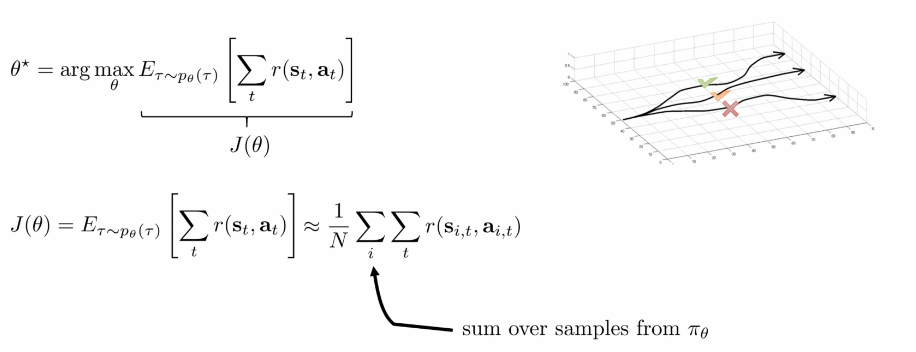
\includegraphics[width=1.0\linewidth]{figures/2020-06-13-111845_916x352_scrot.png}
	\caption{Para coger una estimación de la esperanza, se pueden coger $N$ muestras y
    ponderarlas. Esto nos da un resultado sin bias}
\end{figure}

Teniendo en cuenta la siguiente identidad:
\begin{align}
    \pi_\theta\nabla_\theta\log\pi_\theta(\tau) =
    \nabla_\theta\pi_\theta(\tau)
\end{align}

Se puede hacer lo siguiente:
\begin{align}
        J ( \theta ) &= E _ { \tau \sim \pi _ { \theta } ( \tau ) } [ r ( \tau ) ] = \int \pi _ { \theta }
        ( \tau ) r ( \tau ) d \tau \\
        r(\tau) &= \sum_{t+1}^T r(s_t,a_t)\\
        \nabla _ { \theta } J ( \theta ) &= \int \nabla _ { \theta } \pi _ { \theta } ( \tau ) r ( \tau ) d \tau = \int \pi _ { \theta } ( \tau ) \nabla _ { \theta } \operatorname { log } \pi _ { \theta } ( \tau ) r ( \tau ) d \tau = E _ { \tau \sim \pi _ { \theta } ( \tau ) } [ \nabla _ { \theta } \operatorname { log } \pi _ { \theta } ( \tau ) r ( \tau ) ]
\end{align}

Ahora hay que conocer $\nabla_\theta\log\pi_\theta(\tau)$.

\begin{align}
    \pi _ { \theta } ( s _ { 1 } , a _ { 1 } , \ldots , s _ { T } , a _ { T } ) &= p ( s _ { 1 } )
\prod ^ { T } \pi _ { \theta } ( a _ { t } | s _ { t } ) p ( s _ { t + 1 } | s _ { t } , a _ { t
} )\\
\operatorname { log } \pi _ { \theta } ( \tau ) &= \operatorname { log } p ( s _ { 1 } ) + \sum _ { t = 1 } ^ { T } \operatorname { log } \pi _ { \theta } ( a _ { t } | s _ { t } ) + \operatorname { log } p ( s _ { t + 1 } | s _ { t } , a _ { t } )
\end{align}

Poniendo lo anterior en la ecuación 3.4, se obtiene:

\begin{align}
\nabla _ { \theta } J ( \theta ) = E _ { \tau \sim \pi _ { \theta } ( \tau ) } \left[ ( \sum _ {
    t = 1 } ^ { T } \nabla _ { \theta } \operatorname { log } \pi _ { \theta } ( a _ { t } | s _
    { t } ) ) ( \sum _ { t = 1 } ^ { T } r ( s _ { t } , a _ { t } ) ) \right]
\end{align}

Ya que el primer y último término de 3.6 no dependen de $\theta$.

Por lo que ahora a la hora de calcular las esperanzas mediante muestras, se guardan las
recompensas y los gradientes. 

\begin{align}
\nabla _ { \theta } J ( \theta ) \approx \frac { 1 } { N } \sum _ { i = 1 } ^ { N } ( \sum _ { t = 1 } ^ { T } \nabla _ { \theta } \operatorname { log } \pi _ { \theta } ( a _ { i , t } | s _ { i , t } ) ) ( \sum _ { t = 1 } ^ { T } r ( s _ { i , t } , a _ { i , t } ) )
\end{align}

Para actualizar el modelo se hace ascensor por gradiente:
\begin{align}
    \theta \gets \theta + \alpha\nabla_\theta J(\theta)
\end{align}

\begin{algorithm}
    \caption{REINFORCE}
    \While{no finalice}{
    Muestrear $\{\tau^i\}$ a partir de  $\pi_\theta(a_t|s_t)$ (ejecutar la política)\\
    $ \nabla _ { \theta } J ( \theta ) \approx \sum _ { i } ( \sum _ { t } \nabla _ { \theta }
    \operatorname { log } \pi _ { \theta } ( a _ { t } ^ { i } | s _ { t } ^ { i } ) ) ( \sum _ {
    t } r ( s _ { t } ^ { i } , a _ { t } ^ { i } ) ) $\\
$\theta \gets \theta + \alpha\nabla_\theta J(\theta)$}
\end{algorithm}

\section{¿Qué hace Policy Gradient?}%
\label{sec:_qué_hace_policy_gradient_}

Si se mira la expresión de Policy Gradient se puede ver que es similar a Maximum Likelihood
salvo por el término de las recompensas. Esto quiere decir que en vez de ahce todas las
trayectorias más probables, se hacen más probables aquellas con mayor recompensa, y menos
probables aquellas que obtengan menor recompensa.

La propiedad de Markov no se usa en este algiritmo.

El algoritmo REINFROCE descrito antes no funciona si se aplica tal cual. Policy Gradient
tiene una alta varianza, lo cual es un problema para la estabilidad. Hay varios métodos para
reducirla.

\section{Reducir la varianza: Causalidad}%
\label{sec:reducir_la_varianza_causalidad}

Para este método, se asume que el pasado influye en el futuro y no al revés. Partiendo de la
ecuación 3.8, se agrupan los sumatorios de la siguiente forma equivalente:
\begin{align}
\nabla _ { \theta } J ( \theta ) \approx \frac { 1 } { N } \sum _ { i = 1 } ^ { N } \sum _ { t =
1 } ^ { T } \nabla _ { \theta } \operatorname { log } \pi _ { \theta } ( a _ { i , t } | s _ { i
, t } ) \left( \sum _ { t = 1 } ^ { T } r ( s _ { i , t } , a _ { i , t } ) \right)
\end{align}

Si se observa detenidamente, se puede ver que en el sumatorio de la derecha se está
multiplicando a los gradientes con las recompensas obtenidas en el futuro, lo cual no tiene
mucho sentido. Por ello se puede hacer el siguiente cambio:
\begin{align}
    \nabla _ { \theta } J ( \theta ) \approx \frac { 1 } { N } \sum _ { i = 1 } ^ { N } \sum _ { t
        = 1 } ^ { T } \nabla _ { \theta } \operatorname { log } \pi _ { \theta } ( a _ { i , t } | s _ {
    i , t } ) \left( \sum _ { t' = t } ^ { T } r ( s _ { i , t' } , a _ { i , t' } ) \right)
\end{align}

Simplemente por el hecho de que la suma de las recompensas ahora es menor, el valor de la
varianza es menor. Este método funciona tan bien en la práctica que normalmente se suele
derivar Policy Gradients con el término $\hat{Q}_{i,t} =  \sum _ { t' = t } ^ { T } r ( s _ { i , t' } , a _ { i , t' } )$

\section{Reducir la varianza: Baselines}%
\label{sec:reducir_la_varianza_baselines}

La explicación de que Policy Gradient modifica $\theta$ para preferir los caminos buenos a los
malos no es del todo cierta. Por ejemplo en el caso de que se tenga un escenario en el que
los caminos buenos tengan como recompensa un millón más uno y los malos un millón menos uno, el
ascenso por gradiente hará que todos los caminos sean escogidos por el modelo.

Para arreglar esto, se resta a las recompensas la media de todas las recompensas
obtenidas.

\begin{align}
    \nabla _ { \theta } J ( \theta ) &\approx \frac { 1 } { N } \sum _ { i = 1 } ^ { N } \nabla _ {
\theta } \operatorname { log } \pi _ { \theta } ( \tau ) [ r ( \tau ) - b ]\\
        b &= \frac{1}{N} \sum_{i=1}^{N}r(\tau)
\end{align}

Resulta que matemáticamente la esperanza de esta expresión es la misma que la de original. Se
demuestra calculando la esperanza del nuevo término:
\begin{align}
E [ \nabla _ { \theta } \operatorname { log } \pi _ { \theta } ( \tau ) b ] = \int \pi _ { \theta } ( \tau ) \nabla _ { \theta } \operatorname { log } \pi _ { \theta } ( \tau ) b d \tau = \int \nabla _ { \theta } \pi _ { \theta } ( \tau ) b d \tau = b \nabla _ { \theta } \int \pi _ { \theta } ( \tau ) d \tau = b \nabla _ { \theta } 1 = 0
\end{align}

La esperanza no cambia, pero si que lo hace la varianza. La recompensa media no es el
\textit{baseline} más óptimo, pero es suficientemente bueno. Para calcular el \textit{baseline}
óptimo, se obtiene minimizando la varianza a partir de su definición y derivando con
resepcto a $b$ para obtener el mínimo.

\begin{align}
\left. \begin{array} { l } { \operatorname { Var } [ x ] = E [ x ^ { 2 } ] - E [ x ] ^ { 2 } } \\
{ \nabla _ { \theta } J ( \theta ) = E _ { \tau \sim \pi _ { \theta } ( \tau ) } [ \nabla _ {
\theta } \operatorname { log } \pi _ { \theta } ( \tau ) ( r ( \tau ) - b ) ] } \\ {
\operatorname { Var } = E _ { \tau \sim \pi _ { \theta } ( \tau ) } [ ( \nabla _ { \theta }
\operatorname { log } \pi _ { \theta } ( \tau ) ( r ( \tau ) - b ) ) ^ { 2 } ] - E _ { \tau \sim
\pi _ { \theta } ( \tau ) } [ \nabla _ { \theta } \operatorname { log } \pi _ { \theta } ( \tau )
( r ( \tau ) - b ) ] ^ { 2 } } \end{array} \right.
\end{align}
\begin{align}
    \frac { d \operatorname { Var } } { d b } &= \frac { d } { d b } E [ g ( \tau ) ^ { 2 } ( r ( \tau
    ) - b ) ^ { 2 } ] = \frac { d } { d b } ( E [ g ( \tau ) ^ { 2 } r ( \tau ) ^ { 2 } ] - 2 E [ g (
    \tau ) ^ { 2 } r ( \tau ) b ] + b ^ { 2 } E [ g ( \tau ) ^ { 2 } ] )\\
                                              &= -2E[g(\tau)^2r(\tau)+2bE[g(\tau)^2]] = 0
    \\b &= \frac{E[g(\tau)^2r(\tau)]}{E[g(\tau)^2]} 
\end{align}

Se puede ver que es la esperanza de la recompensa pero ponderada por las magnitudes de los
gradientes. $b$ es un vector para cada parámetro del modelo a optimizar, lo que proporciona un
\textit{baseline} para cada parámetro.

\section{Derivación de Policy Gradient con Importance Sampling}%
\label{sec:derivación_de_policy_gradient_con_importance_sampling}

\begin{align}
J ( \theta ^ { \prime } ) = E _ { \tau \sim \pi _ { \theta } ( \tau ) } [ \frac { \hat { \pi _ {
\theta ^ { \prime } } ( \tau ) } } { \pi _ { \theta } ( \tau ) } r ( \tau ) ]\\
\nabla _ { \theta ^ { \prime } } J ( \theta ^ { \prime } ) = E _ { \tau \sim \pi _ { \theta } (
\tau ) } [ \frac { \nabla _ { \theta ^ { \prime } } \pi _ { \theta ^ { \prime } } ( \tau ) } {
\pi _ { \theta } ( \tau ) } r ( \tau ) ] = E _ { \tau \sim \pi _ { \theta } ( \tau ) } [ \frac {
\pi _ { \theta ^ { \prime } } ( \tau ) } { \pi _ { \theta } ( \tau ) } \nabla _ { \theta ^ {
\prime } } \operatorname { log } \pi _ { \theta ^ { \prime } } ( \tau ) r ( \tau ) ]
\end{align}

En el caso de que se estime localmente: $\theta=\theta':\;\;\nabla_\theta J(\theta) = E_{\tau
\sim \pi_\theta(\tau)}[\nabla_\theta\log\pi_\theta(\tau)r(\tau)]$ se obtiene la expresión que nos
es familiar. En el caso de que sea \textit{off-policy}, se obtiene lo siguiente:

\begin{align}
    \nabla _ { \theta ^ { \prime } } J ( \theta ^ { \prime } ) &= E _ { \tau \sim \pi _ { \theta
    } ( \tau ) } [ \frac { \pi _ { \theta ^ { \prime } } ( \tau ) } { \pi _ { \theta } ( \tau ) }
    \nabla _ { \theta ^ { \prime } } \operatorname { log } \pi _ { \theta ^ { \prime } } ( \tau )
    r ( \tau ) ]\\
&= E _ { \tau \sim \pi _ { \theta } ( \tau ) } [ ( \prod _ { t = 1 } ^ { T } \frac { \pi _ { \theta ^ { \prime } } ( a _ { t } | s _ { t } ) } { \pi _ { \theta } ( a _ { t } | s _ { t } ) } ) ( \sum _ { t = 1 } ^ { T } \nabla _ { \theta ^ { \prime } } \operatorname { log } \pi _ { \theta ^ { \prime } } ( a _ { t } | s _ { t } ) ) ( \sum _ { t = 1 } ^ { T } r ( s _ { t } , a _ { t } ) ) ]
\end{align}

En el caso de que $T$ sea muy grande, lo que pasa es que
$\frac{\pi_{\theta'}(\tau)}{\pi_{\theta}(\tau)}$ puede ser exponencialmente pequeño o grande, lo
cual puede hacer que los gradientes sean cercanos a nulos o exploten, incrementando la
varianza. Se puede intentar aplicar la causalidad, que aunque alivia esto no resuelve el problema:

\begin{align}
\pi _ { \theta } ( \tau ) [ \sum _ { t = 1 } ^ { T } \nabla _ { \theta ^ { \prime } } \operatorname { log } \pi _ { \theta ^ { \prime } } ( a _ { t } | s _ { t } ) ( \prod _ { t ^ { \prime } = 1 } ^ { t } \frac { \pi _ { \theta ^ { \prime } } ( a _ { t ^ { \prime } } | s _ { t ^ { \prime } } ) } { \pi _ { \theta } ( a _ { t ^ { \prime } } | s _ { t ^ { \prime } } ) } ) ( \sum _ { t ^ { \prime } = t } ^ { T } r ( s _ { t ^ { \prime } } , a _ { t ^ { \prime } } ) ( \prod _ { t ^ { \prime \prime } = t } ^ { t ^ { \prime } } \frac { \pi _ { \theta ^ { \prime } } ( a _ { t ^ { \prime \prime } } | s _ { t ^ { \prime \prime } } ) } { \pi _ { \theta } ( a _ { t ^ { \prime \prime } } | s _ { t ^ { \prime \prime } } ) } ) ) ]
\end{align}

También puede interesarnos actualizar nuestro modelo con muestras obtenidas de una política
parecida a la que se tiene actualmente, para lo cual se puede usar la siguiente expresión:

\begin{figure}[htpb]
	\centering
	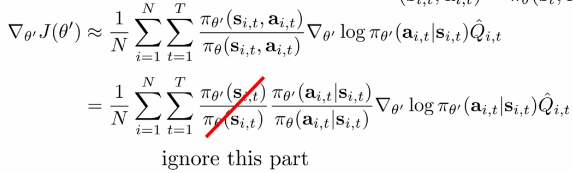
\includegraphics[width=0.8\linewidth]{figures/2020-06-13-131824_573x173_scrot.png}
\end{figure}

\section{Implementar Policy Gradient con diferenciación automática}%
\label{sec:implementar_policy_gradient_con_diferenciación_automática}

Es muy ineficiente calcular los gradientes, aplicarle el logaritmo y hacer el sumatorio. En su
lugar se tiene que construir un grafo de tal manera que la derivada de ese grafo es el
gradiente de la política.

Como las librería incluyen ya ML como objetivo:
\begin{align}
\nabla _ { \theta } J _ { ML } ( \theta ) \approx \frac { 1 } { N } \sum _ { i = 1 } ^ { N } \sum _ { t = 1 } ^ { T } \nabla _ { \theta } \operatorname { log } \pi _ { \theta } ( a _ { i , t } | s _ { i , t } ) \quad J _ { ML } ( \theta ) \approx \frac { 1 } { N } \sum _ { i = 1 } ^ { N } \sum _ { t = 1 } ^ { T } \operatorname { log } \pi _ { \theta } ( a _ { i , t } | s _ { i , t } )
\end{align}

Lo que se hace es implementar una pseudo-pérdida de forma que su derivada sea el gradiente de
la política:

\begin{align}
\tilde { J } ( \theta ) \approx \frac { 1 } { N } \sum _ { i = 1 } ^ { N } \sum _ { t = 1 } ^ { T } \operatorname { log } \pi _ { \theta } ( a _ { i , t } | s _ { i , t } ) \hat { Q } _ { i , t }
\end{align}

Un ejemplo en Tensorflow sería el siguiente:

\begin{figure}[H]
    \caption{Maximum likelihood}
	\centering
	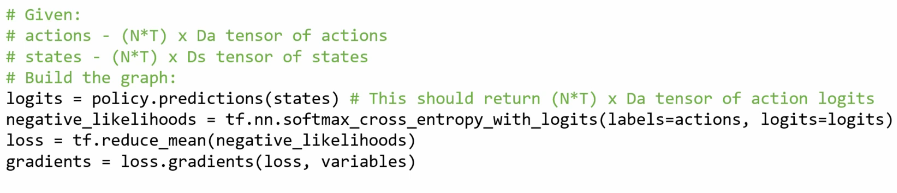
\includegraphics[width=0.8\linewidth]{figures/2020-06-13-132416_897x193_scrot.png}
\end{figure}

\begin{figure}[H]
	\centering
	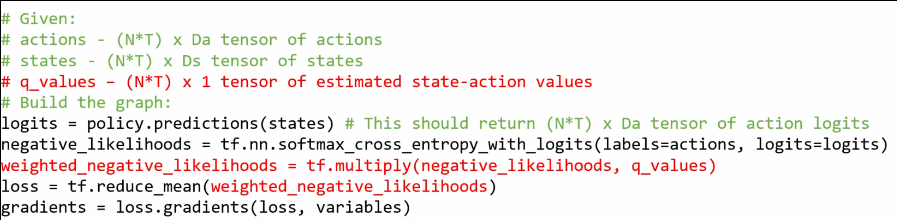
\includegraphics[width=0.8\linewidth]{figures/2020-06-13-132508_897x220_scrot.png}
	\caption{Policy Gradient}
\end{figure}

\section{Policy Gradients en la práctica}%
\label{sec:policy_gradients_en_la_práctica}

\begin{itemize}
    \item Los gradientes tienen una alta varianza, al contrario que en aprendizaje
        supervisado. Los gradientes serán muy ruidosos.
    \item Normalmente se usan \textit{batches} grandes
    \item Optimizar los \textit{learning rates} es difícil. ADAM y otros similares pueden
        aliviar un poco esto.
\end{itemize}

\section{Resumen}%
\label{sec:resumen}

\begin{itemize}
    \item Policy Gradients es \textit{on-policy}
    \item Se puede derivar una variante \textit{off-policy}
        \begin{itemize}
            \item Usando Importance Sampling
            \item Escalado exponencial con respecto a $T$.
            \item Se puede ignorar parte de los pesos.
        \end{itemize}
    \item Se puede implementar con diferenciación automática.
\end{itemize}
